\documentclass[a4paper, 12pt]{article}
\usepackage[T1]{fontenc}
\usepackage{lmodern}
\usepackage{pdfpages}
\usepackage{color}
\usepackage{steinmetz}
\usepackage{amsfonts}
\usepackage{epstopdf}
\usepackage{matlab}
%\documentclass{book}
\usepackage{blindtext}
\usepackage{hyperref}
\usepackage[brazil]{babel}
\usepackage{amssymb}
\usepackage[utf8]{inputenc}
\usepackage{amsmath}
\usepackage{indentfirst}
\usepackage{graphicx}
\usepackage{multicol,lipsum}
\usepackage[a4paper,
top=3cm, left=3cm, bottom=3cm, right=3cm]{geometry}
\usepackage{setspace}
\usepackage{multirow}
\usepackage{float}
\usepackage[dvipsnames]{xcolor}
\usepackage[table]{xcolor}
%\usepackage{pdflscape}
\usepackage[DIV=15]{typearea}
\usepackage[nottoc]{tocbibind}
\usepackage[sort,numbers]{natbib}
%\usepackage{cite}
\usepackage{matlab}

\usepackage[utf8]{inputenc}
\usepackage[T1]{fontenc}
\usepackage{lmodern}
\usepackage{graphicx}
\usepackage{color}
\usepackage{hyperref}
\usepackage{amsmath}
\usepackage{amsfonts}
\usepackage{epstopdf}
\usepackage[table]{xcolor}
\usepackage{matlab}


\documentclass[letterpaper]{article}
% bib pack %%%%%%%%%%%%%%%%%%%%%%%%%%%%%%%%%%%%%%%%%%%%%%%%%%%%%%%%%%%%%%%%%%%%%
\usepackage[utf8]{inputenc}
\usepackage{geometry}
    \geometry{left=3cm,right=2cm,top=2cm,bottom=2cm}
%
\usepackage[spanish]{babel}
%
\usepackage[fixlanguage]{babelbib}
    \bibliographystyle{babunsrt}
%
\usepackage{url}

\begin{document}
%\maketitle

\begin{titlepage}
	\begin{center}
		

\vspace{10pt}
%\begin{figure}[H][!ht]
%\centering
%
\includegraphics{puc-rio-logo.png}

%\end{figure}
\begin{figure}[!ht]
\centering

\includegraphics{images/puc-rio-logo.png}
\end{figure}
\huge{Instrumentação Eletrônica}
        \vspace{70pt}
        
		\textbf{ENG1027}
		\textbf{\large{\\ }}
		
		\vspace{30pt}
		\textbf{\small{\\Transistores}}
		\vspace{75pt}
		
	\end{center}
	
	\begin{flushleft}
		\begin{tabbing}
			Alunos\qquad\qquad\=\>Paloma Sette - 1621595\\
			\> Renan Sued - 1621618\\
			\> Luiz Manoel - 1713129 \\
                \> \\
			Professor\>Igor Braga de Paula\\
	\end{tabbing}
		  
	\end{flushleft}
	\begin{center}
		%\vspace{\fill}
		\vspace{215pt}
		Rio de Janeiro, 22 de Junho de 2023
	\end{center}
\end{titlepage}
%%%%%%%%%%%%%%%%%%%%%%%%%%%%%%%%%%%%%%%%%%%%%%%%%%%%%%%%%%%



\newpage
\pagenumbering{arabic}

\newpage

%\newcommand{\listequationsname}{Lista de Equações}
%\newlistof{myequations}{equ}{\listequationsname}
%\newcommand{\myequations}[1]{%
%\addcontentsline{equ}{myequations}{\protect\numberline{\theequation}#1}\par}

%\listofmyequations
%%%%%%%%%%%%%%%%%%%%%%%%%%%%%%%%%%%%%%%%%%%%%%%%%%%%%%%%%%%
\newpage
\tableofcontents
\thispagestyle{empty}

\newpage
\pagenumbering{arabic}

\newpage

%\newcommand{\listequationsname}{Lista de Equações}
%\newlistof{myequations}{equ}{\listequationsname}
%\newcommand{\myequations}[1]{%
%\addcontentsline{equ}{myequations}{\protect\numberline{\theequation}#1}\par}

%\listofmyequations
\newpage


\newpage

\listoffigures
\thispagestyle{empty}

\newpage
%%%%%%%%%%%%%%%%%%%%%%%%%%%%%%%%%%%%%%%%%%%%%%%%%%%%%%%%%
%%%%%%%%%%%%%%%%%%%%%%%%%%%%%%%%%%%%%%%%%%%%%%%%%%%

\newpage

\thispagestyle{empty}

\newpage


\section*{Introdução}
Este relatório refere-se à sequência de atividades relativas à Transistores, da disciplina de Instrumentação Eletrônica (ENG1027) de 2023.1. \\

Descreveremos os resultados ocorridos nas simulações propostas, com base no transistor MPS3903.\\

\section{Exercício}

Com base no que foi visto nas aulas sobre funcionamento de transistores pede-se para projetar e 
simular alguns circuitos usando o transistor MPS3903, cujo datasheet encontra-se anexo. Os circuitos 
que serão projetados para trabalhar a 25ºC e possuem as seguintes especificações: \\

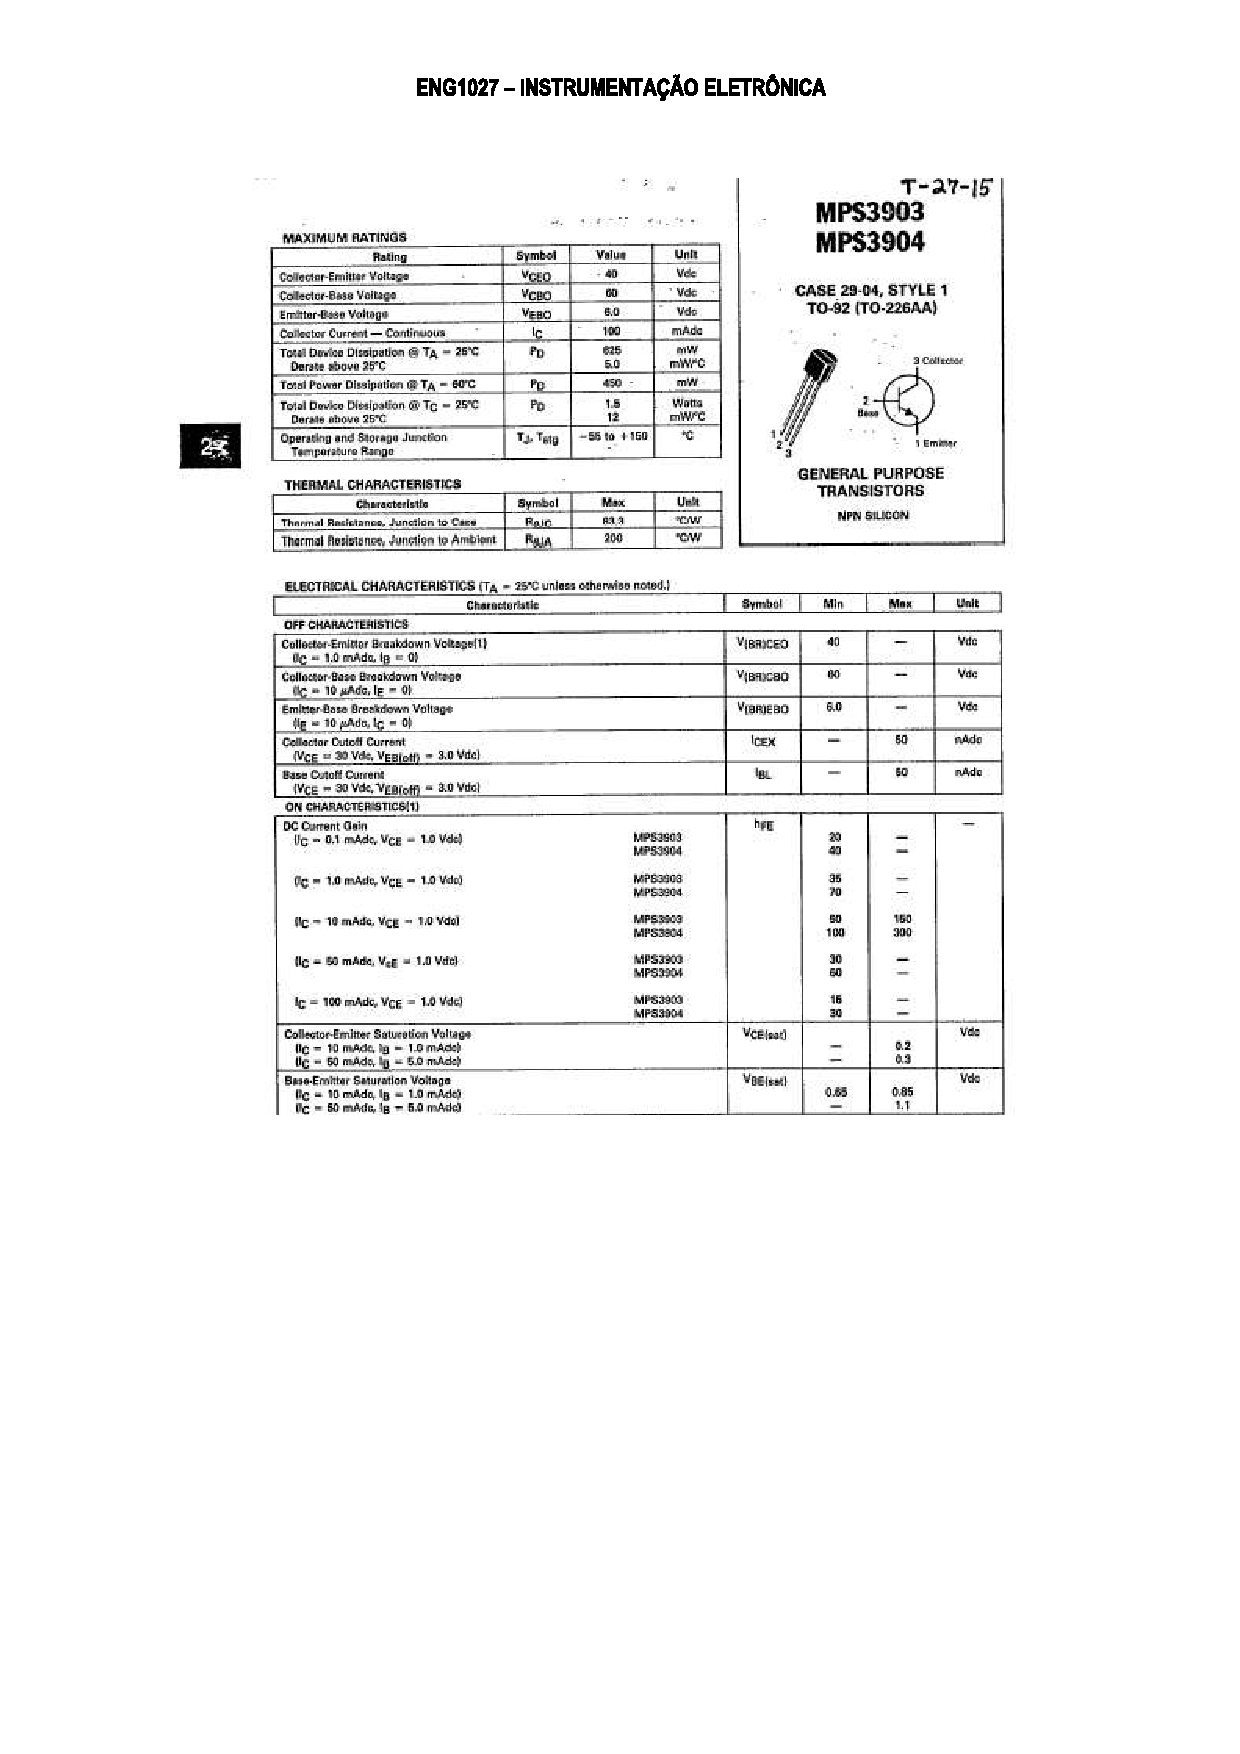
\includepdf[pages={1, 2, 3}, pagecommand={\section{Anexo}}, 
    scale=0.9, 
    offset=0mm -10mm, 
    pagecommand={\thispagestyle{plain}},
    clip, 
    trim=10mm 10mm 10mm 10mm,
    center]{transistores.pdf}

\subsection{Ex. 1}
O circuito deve permitir o controle da corrente em uma carga resistiva a partir de um sinal de  corrente. O sinal de controle tem corrente muito baixa (pode variar de 0 até no máx 500$\mu A$). A carga está ligada a uma fonte de 12V e a corrente na carga deve ser controlada na faixa entre 5mA e 50mA, sendo que esses valores correspondem a corrente mínima e máxima respectivamente. 

\subsubsection{Projete esse circuito (escolha componentes adequados) e faça os cálculos teóricos (incluir memorial de cálculo detalhado)}

Para projetar o circuito que permite o controle da corrente em uma carga resistiva usando o transistor MPS3903, , é necessário fazermos algumas considerações:\\

\textbf{O Transistor}: O transistor MPS3903 é um transistor NPN de baixa potência. Verificamos se suas especificações atendem aos requisitos do circuito, como corrente máxima e ganho.\\ \\

\textbf{Determinação da corrente de base:} No caso de um transistor NPN como o MPS3903, a corrente de base é responsável por controlar a corrente de coletor. O objetivo é garantir que o transistor esteja devidamente acionado e na região de operação desejada.\\ 

Para calcular a corrente de base necessária para uma corrente de coletor específica, precisamos levar em consideração o ganho de corrente do transistor (hFE), que é uma relação entre a corrente de coletor e a corrente de base.\\

Entao, fazemos a nossa abordagem:

\begin{itemize}
    \item Determinar a corrente de coletor desejada: No nosso caso, precisamos que a corrente na carga seja controlada na faixa entre 5mA e 50mA.
    \item Determinando o ganho de corrente (hFE): Como queremos trabalhar a 25ºC e nossa faixa operacional de corrente $I_c$ precisa ser de 5mA a 50mA, pelo gráfico de hFE x $I_c$ do datasheet, podemos traçar uma linha vertical sobre os valores de 5mA e 50mA e depois outra linha horizontal onde há a interseção entre as linhas verticais e as curvas na área de 25ºC:
    \begin{figure}[H]
    \centering
    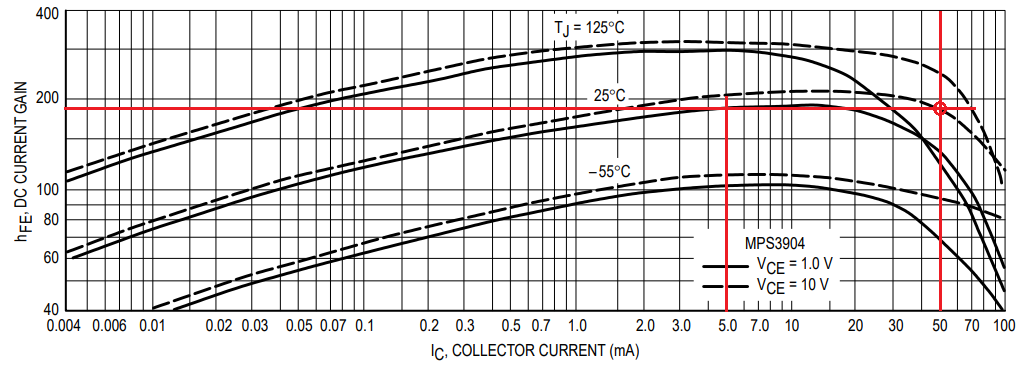
\includegraphics[scale = 0.45]{images/ganho.png}
    \label{filtro1}
    \caption{Ganho de corrente em função da corrente de carga}
    \end{figure}

    Neste caso, podemos estimar que nosso ganho ficará em torno de 200.
        
    \item calculando a corrente de base necessária:
        \begin{equation*}
            I_b = \frac{I_c}{hFE} = \frac{5mA}{200} = 25 \mu A
        \end{equation*}
        \end{itemize}
    
        \begin{equation*}
            I_b = \frac{I_c}{hFE} = \frac{50mA}{200} = 250 \mu A
        \end{equation*}
        \end{itemize}

        Neste caso, a corrente de base deverá atuar em uma faixa de $25\mu A $ a $250 \mu A$. \\ \\

\textbf{Cálculo da resistência de base:} A resistência de base será usada para limitar a corrente de base. Sabendo que a tensão de base-emissor de um transistor NPN é de aproximadamente 0,7V, teremos:

\begin{equation*}
    R_b = \frac{V_{be}}{I_b} = \frac{0,7V}{25\mu A} = 28,0k \Omega
\end{equation*}

\begin{equation*}
    R_b = \frac{V_{be}}{I_b} = \frac{0,7V}{250\mu A} = 2,80k \Omega
\end{equation*}

Neste caso, a resistência de base será um valor comercial dentro da faixa de $2,8k\Omega - 28k\Omega$. \\ \\


\textbf{Cálculo do valor da resistência de carga:} Como a carga deve ser controlada na faixa entre 5mA e 50mA, escolheremos um valor para a resistência de carga ($R_c$) com base nessas condições.\\

$V_{in} = 12V$ ;\\
$I_{cmin} = 5mA$ ;\\
$I_{cmax} = 50mA$

\begin{equation*}
    R_{cmin} = \frac{V_{in}}{I_{cmin}} =\frac{12V}{50mA} = 240 \Omega
\end{equation*}
\begin{equation*}
    R_{cmax} = \frac{V_{in}}{I_{cmin}} =\frac{12V}{5mA} = 2,40k \Omega
\end{equation*}



\subsubsection{Simule o circuito. Faça um gráfico a partir da simulação com a curva de carga do transistor.}

De acordo com o estimado, nossa curva de carga ficaria da seguinte forma:

    \begin{figure}[H]
    \centering
    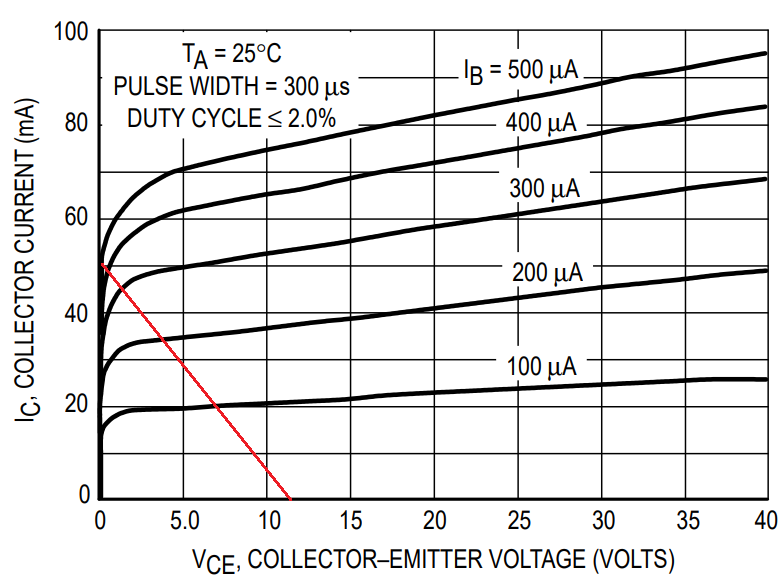
\includegraphics[scale = 0.5]{images/curva_carga.png}
    \caption{Curva de carga}
    \end{figure}

Utilizamos o LTSpice para simular o circuito, a fim de gerar os resultados através da curva plotada.

    \begin{figure}[H]
    \centering
    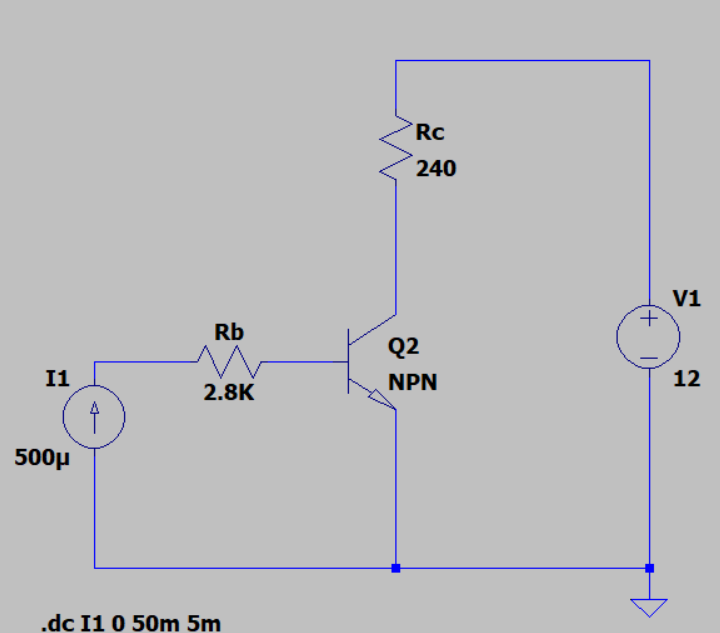
\includegraphics[scale = 0.6]{images/circuito_LTSPICE.png}
    \caption{Simulação no LTSpice}
    \end{figure}

Inserimos os valores dos componentes de acordo com o que foi calculado anteriormente. Vale ressaltar que, no LTSpice, infelizmente não encontramos o transistor em questão. Fizemos alguns testes utilizando transistores similares e, por fim, um transistor genérico, o que nos gerou o mesmo resultado em todas as simulações realizadas. 
Portanto, abaixo segue o resultado gráfico:

    \begin{figure}[H]
    \centering
    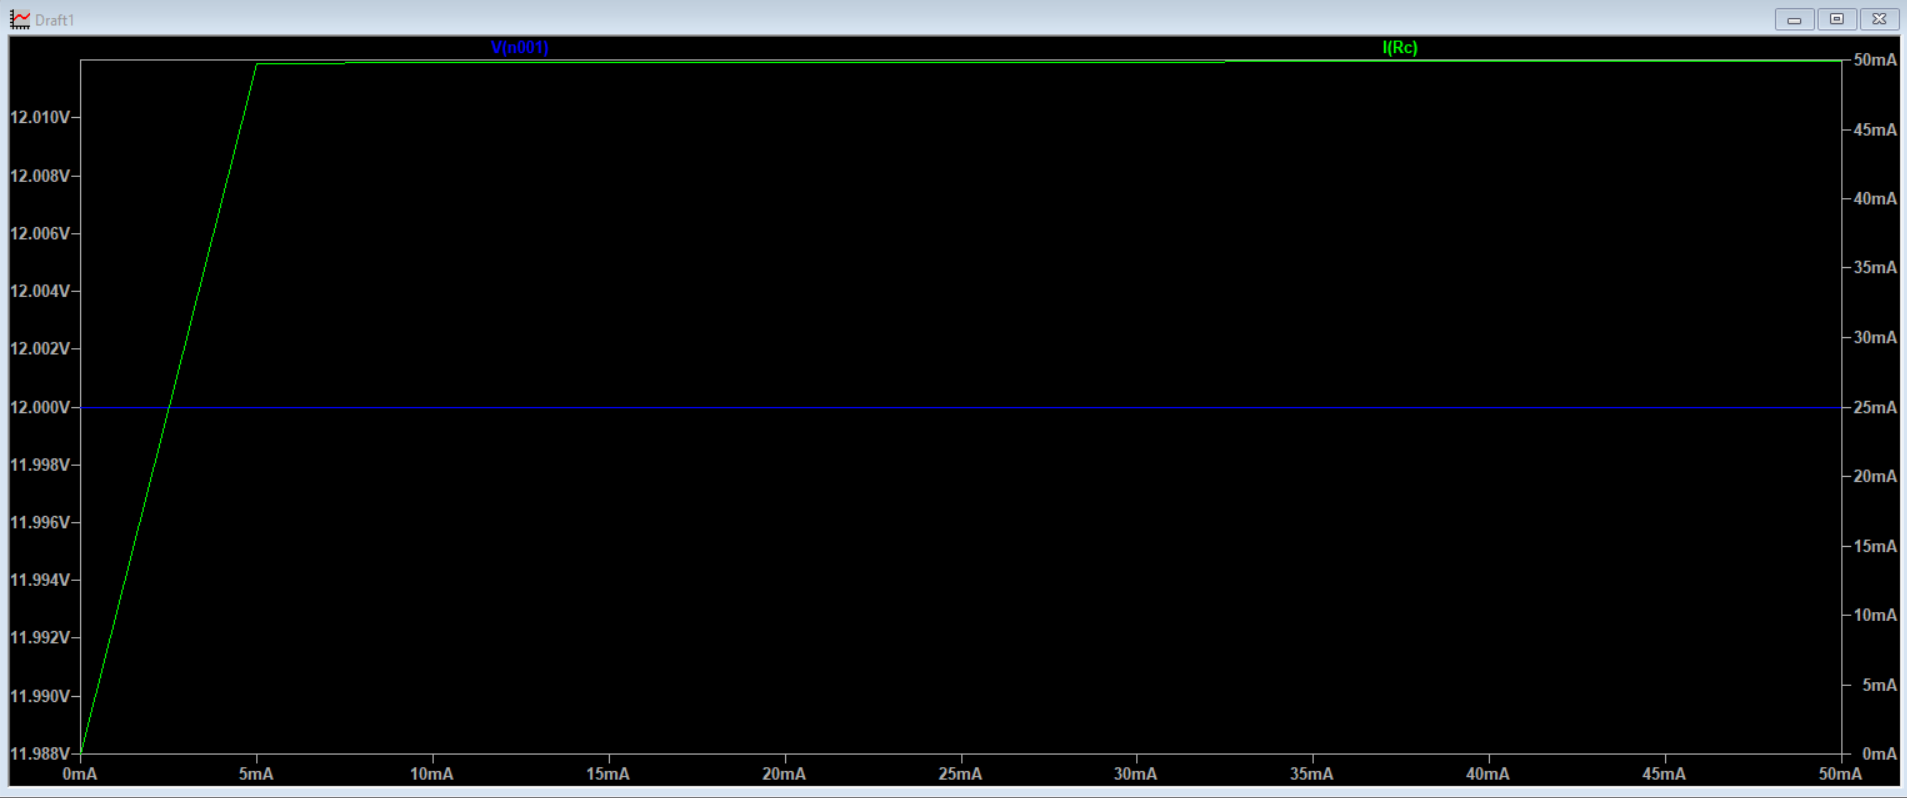
\includegraphics[scale = 0.4]{images/grafico1.png}
    \caption{Gráfico representante da curva de carga}
    \end{figure}


\subsubsection{ Comparando os resultados}
Embora a configuração do gráfico esteja diferente da que consta no datasheet e também das que foram vistas em vídeoaulas com o TopSpice, podemos concluir que a curva gerada condiz com o que esperávamos. Ou seja, podemos verificar que, para uma tensão de 12V gerada pela fonte, com a corrente do emissor tendo valor nulo, teremos que a ddp será máxima e, portanto, atingiremos o valor de $I_{cmax}$.  



\newpage
\subsection{Ex. 2}
 Usando os mesmos requerimentos especificações do circuito acima, com exceção da corrente do 
máxima do sinal de controle, projete um novo circuito que confira um ganho de corrente da ordem de 2000. Dica: usar dois transistores. Simular o circuito e mostrar curva de carga teórica e simulada.

    \begin{figure}[H]
    \centering
    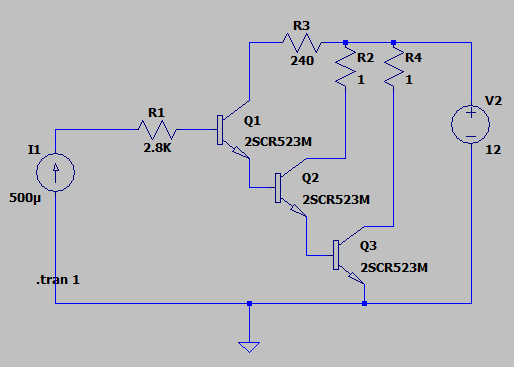
\includegraphics[scale = 0.8]{images/circuito_1.png}
    \caption{Circuito com o ganho de 2.800}
    \end{figure}
Utilizamos 3 transistor para conseguir o ganho de 2800 de corrente no acionamento. Como podemos ver no gráfico anterior.

No gráfico abaixo podemos obsevar a curva de carga do primeiro transistor Q1.

    \begin{figure}[H]
    \centering
    
\includegraphics[scale = 0.4]{images/grafico_2_1.png}
    \caption{Curvade carga Q1 (vermelha)}
    \end{figure}
    
No gráfico abaixo podemos observar a curva de carga do primeiro transistor Q2 e Q3, com ganhos de 42x e 31x respectivamente.

    \begin{figure}[H]
    \centering
    
\includegraphics[scale = 0.4]{images/grafico_2_2.png}
    \caption{Gráfico Q2 (verde) e Q3 (azul) com ganhos totais de 2.800}
    \end{figure}

Por fim a junção dos 3 transistors nos concedeu um ganho de 2800, porem esse ganho foi cascateado conforme o circuito foi passando, isso dado a fonte de 12v juntamente com o divisor de corrente que está alimentando os coletores de cada transistor.










\begin{equation*}
    X = 2\phase{10^ {\circ}}
\end{equation*}









\newpage



% REFERENCIAS %%%%%%%%%%%%%%%%%%%%%%%%%%%%%%%%%%%%%%%%%%%%%%%%%%%%%%%%%%%%%%


\end{document}